%% Copernicus Publications Manuscript Preparation Template for LaTeX Submissions
\documentclass[gmd, manuscript]{copernicus}

\usepackage{pdfpages}
\usepackage{booktabs}
\usepackage{pdflscape}

\usepackage{multirow}
\usepackage{makecell}
\graphicspath{{./}}
\newcommand{\num}[1]{#1}
\newsavebox{\benchmarktablebox}
\newcommand{\benchmarktablefont}{\normalsize}
\newcommand{\fitwidth}[1]{%
  \sbox{\benchmarktablebox}{#1}%
  \ifdim\wd\benchmarktablebox>\linewidth
    \resizebox{\linewidth}{!}{\usebox{\benchmarktablebox}}%
  \else
    \usebox{\benchmarktablebox}%
  \fi
}


\newif\ifbenchmarklandscape
\AddToHook{shipout/foreground}{%
  \ifbenchmarklandscape
    \AtPageLowerLeft{%
      \put(\LenToUnit{\dimexpr\paperwidth-1.2cm\relax},\LenToUnit{0.5\paperheight}){\rotatebox{90}{\thepage}}%
    }%
  \fi
}
\newenvironment{benchmarklandscape}{%
  \clearpage
  \benchmarklandscapetrue
  \pagestyle{empty}%
  \begin{landscape}%
}{%
  \end{landscape}%
  \benchmarklandscapefalse
  \pagestyle{plain}%
  \clearpage
}

\emergencystretch=2em

\begin{document}

\title{Kramer Annulus Stokes Benchmark Using Underworld3}

\Author[1][gthyagi@gmail.com]{Thyagarajulu}{Gollapalli}
\Author[1]{Underworld}{Team}

\affil[1]{Research School of Earth Sciences, Australian National University, Canberra, ACT, Australia}

\runningtitle{Kramer annulus Stokes benchmark in Underworld3}
\runningauthor{Gollapalli}

\received{}
\pubdiscuss{}
\revised{}
\accepted{}
\published{}

\firstpage{1}

\maketitle

\begin{abstract}
We reproduce the annulus benchmark of \citet{kramer2021} using Underworld3
(UW3). The benchmark solves incompressible, isoviscous Stokes flow in a
two-dimensional cylindrical shell with analytical forcing and analytical
velocity and pressure solutions. It tests curved boundaries, pressure
normalisation, free-slip and zero-slip velocity conditions, and both smooth and
interface-localised density forcing. The UW3 calculations use
\(P_2\times P_1\) Taylor--Hood finite elements on refined annulus meshes with
nominal cell sizes \(h=1/8,\ldots,1/256\). Errors are measured using relative
volume \(L_2\) norms for velocity and pressure. Smooth forcing cases recover
approximately second-order pressure convergence and systematic second-order or
better velocity convergence over the tested refinement range. Delta-function
forcing cases show reduced but regular convergence, with velocity rates near
\(O(h^{1.5})\) and pressure rates near \(O(h^{0.5})\), consistent with the
reduced regularity of interface-localised buoyancy forcing. These results
verify the UW3 annulus Stokes implementation for curved-shell geometry and for
both boundary-condition families considered in the Kramer benchmark.
\end{abstract}

\introduction

Analytical benchmarks are central to verification of geodynamic Stokes-flow
codes because they separate discretisation and implementation errors from
uncertainty in the reference solution. Annulus benchmarks are particularly useful
for mantle-convection software: they include curved boundaries and polar
coordinate forcing while remaining cheaper and easier to inspect than full
spherical-shell calculations.

The analytical solutions of \citet{kramer2021} provide a family of mantle-flow
benchmarks in cylindrical and spherical shells. In the cylindrical annulus, the
solutions include free-slip and zero-slip boundary conditions, smooth volumetric
forcing, and delta-function forcing on an internal circular interface. This
combination exercises several aspects of a finite-element Stokes implementation:
velocity--pressure coupling, pressure gauge removal, curved-domain integration,
normal and tangential boundary constraints, and the treatment of fields with
limited regularity.

Here we summarise the UW3 reproduction of the Kramer annulus benchmark. The
article is based on the corresponding UW3 benchmark report and uses only the
existing generated figures and tables. The goal is to document the mathematical
setup, numerical choices, error definitions, and observed convergence behaviour
in a concise Copernicus-style manuscript.

\section{Governing Equations and Benchmark Solution}

The benchmark solves the steady incompressible Stokes equations in a
two-dimensional annulus \(\Omega=\{(r,\theta):R_-\leq r\leq R_+\}\):
\begin{subequations}
\begin{align}
  -\nabla\cdot\boldsymbol{\sigma} &= \rho\mathbf{g}, \\
  \nabla\cdot\mathbf{u} &= 0,
\end{align}
\end{subequations}
where \(\mathbf{u}\) is velocity, \(p\) is pressure, \(\rho\) is density, and
\(\mathbf{g}\) is gravitational acceleration. The stress tensor is
\begin{equation}
  \boldsymbol{\sigma}
  =
  -p\mathbf{I}
  +2\eta\boldsymbol{\varepsilon}(\mathbf{u}),
  \qquad
  \boldsymbol{\varepsilon}(\mathbf{u})
  =
  \frac{1}{2}\left(\nabla\mathbf{u}+\nabla\mathbf{u}^{T}\right),
\end{equation}
with constant viscosity \(\eta\).

Following \citet{kramer2021}, the annulus radii are
\[
  R_- = 1.22,
  \qquad
  R_+ = 2.22.
\]
For the interface-localised cases, the internal density interface is located at
\[
  R_{\mathrm{int}} = 2.0.
\]
The analytical forcing is separated into azimuthal and radial parts. Smooth
cases use a density perturbation proportional to
\begin{equation}
  \left(\frac{r}{R_+}\right)^k\cos(n\theta),
\end{equation}
where \(k\) controls the radial structure and \(n\) controls the azimuthal
wavenumber. Delta-function cases use an interface forcing proportional to
\begin{equation}
  \delta(r-R_{\mathrm{int}})\cos(n\theta).
\end{equation}
The full analytical velocity and pressure fields are those derived by
\citet{kramer2021}; the UW3 implementation evaluates these closed-form
solutions to define the forcing, impose the benchmark boundary conditions, and
measure numerical error.

\section{Numerical Setup}

The UW3 calculations use \(P_2\times P_1\) Taylor--Hood elements, with
quadratic velocity and continuous linear pressure. This mixed pair is a standard
choice for incompressible Stokes flow and is expected to provide robust pressure
behaviour for smooth solutions \citep{girault1986,boffi2013}. The pressure
nullspace is removed before error evaluation because incompressible Stokes flow
determines pressure only up to an additive constant.

The verification suite contains four benchmark groups (Table~\ref{tab:cases}).
Cases 1 and 2 use free-slip boundaries, while Cases 3 and 4 use zero-slip
boundaries. Cases 1 and 3 use delta-function forcing on the internal interface;
Cases 2 and 4 use smooth volumetric forcing. The tested nominal mesh sizes are
\(h=1/8,\ldots,1/256\).

\begin{table}[H]
\centering
\caption{Kramer annulus benchmark cases used in the UW3 verification runs.}
\label{tab:cases}
\begin{tabular}{cllll}
\toprule
Case & Forcing & Boundary condition & Parameters & Resolutions \\
\midrule
1 & Delta function & Free slip & \(n=2,8,32\) & \(1/8\)--\(1/256\) \\
2 & Smooth & Free slip & \(n=2,8,32;\ k=2,8\) & \(1/8\)--\(1/256\) \\
3 & Delta function & Zero slip & \(n=2,8,32\) & \(1/8\)--\(1/256\) \\
4 & Smooth & Zero slip & \(n=2,8,32;\ k=2,8\) & \(1/8\)--\(1/256\) \\
\bottomrule
\end{tabular}
\end{table}

Figure~\ref{fig:density} shows representative analytical density perturbations.
Increasing \(n\) increases the angular complexity of the benchmark solution.
For smooth forcing, increasing \(k\) changes the radial weighting of the density
field. For delta-function forcing, the density is concentrated on the internal
interface and therefore reduces solution regularity relative to the smooth
cases.

\begin{figure}[H]
    \centering
    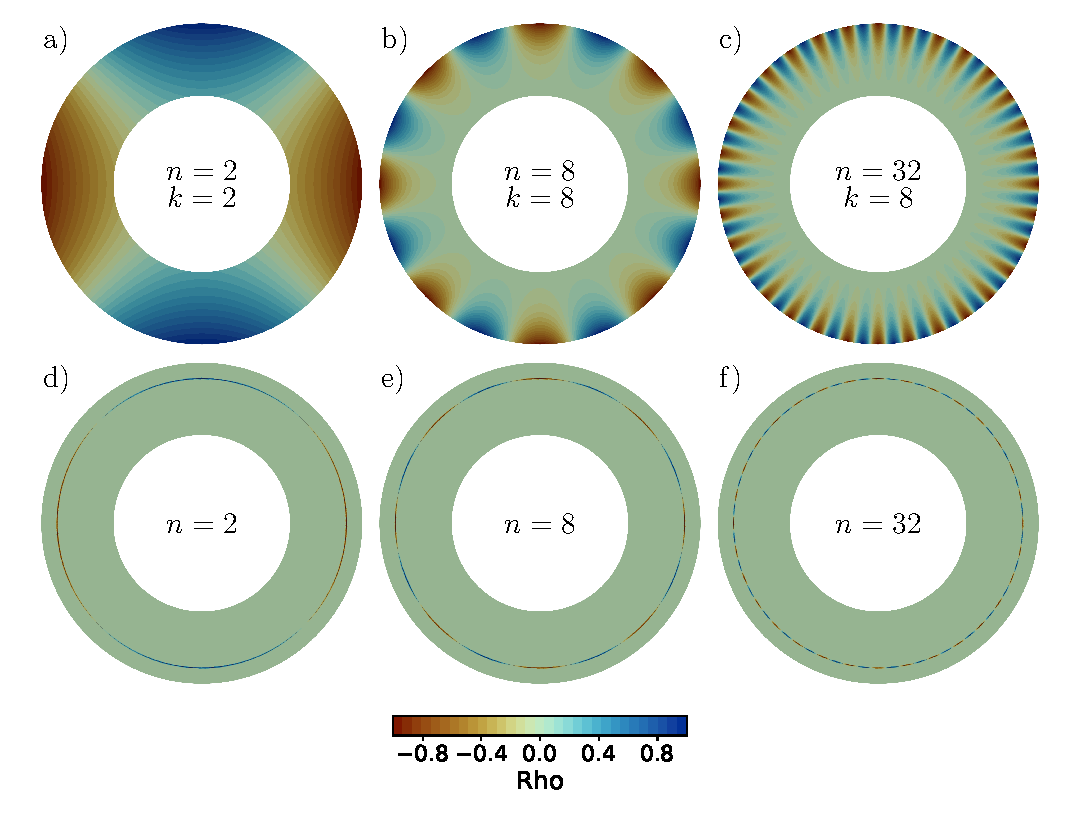
\includegraphics[width=0.98\linewidth]{figure_1_kramer_annulus_rho_ana.pdf}
    \caption{Analytical density perturbations for the Kramer annulus benchmark.
    The upper row shows smooth forcing and the lower row shows delta-function
    forcing. Columns correspond to increasing azimuthal complexity.}
    \label{fig:density}
\end{figure}

\section{Error Metrics}

Velocity and pressure errors are reported as relative volume \(L_2\) norms. For
a numerical field \(q_h\) and analytical reference field \(q^*\), the relative
error is
\begin{equation}
  E_{L_2}^{\mathrm{rel}}(q)
  =
  \left(
  \frac{\int_{\Omega}|q_h-q^*|^2\,\mathrm{d}\Omega}
       {\int_{\Omega}|q^*|^2\,\mathrm{d}\Omega}
  \right)^{1/2}.
\end{equation}
Thus the table and figure labels use \(E_{L_2}^{\mathrm{rel}}(\mathbf{u})\)
for velocity and \(E_{L_2}^{\mathrm{rel}}(p)\) for pressure.
For two consecutive refinements with characteristic mesh sizes \(h_1\) and
\(h_2\), the observed convergence rate is
\begin{equation}
  \alpha
  =
  \frac{\log(E_{h_1}/E_{h_2})}{\log(h_1/h_2)}.
\end{equation}
With uniform halving of the nominal mesh size, this reduces to
\(\alpha=\log_2(E_{h_1}/E_{h_2})\).

\section{Results}

The convergence results are shown in Fig.~\ref{fig:convergence}. For the smooth
forcing cases, pressure errors converge close to \(O(h^2)\) for both free-slip
and zero-slip boundary conditions. Velocity errors converge systematically and
are approximately second order for \(n=2\) and \(n=8\). The high-wavenumber
\(n=32\) smooth cases show larger error constants and stronger pre-asymptotic
behaviour, but the rates decrease toward the expected refined-mesh trend as the
solution becomes better resolved.

The delta-function forcing cases exhibit lower rates. Velocity convergence
approaches \(O(h^{1.5})\), while pressure convergence approaches \(O(h^{0.5})\)
for both free-slip and zero-slip boundaries. This behaviour is expected for the
Kramer benchmark because the Green's-function solution associated with
interface-localised forcing is less regular than the smooth volumetric-forcing
solution \citep{kramer2021}. The reduced pressure rate is therefore interpreted
as a property of the benchmark solution regularity rather than as a failure of
the Stokes solver.

\begin{figure}[H]
    \centering
    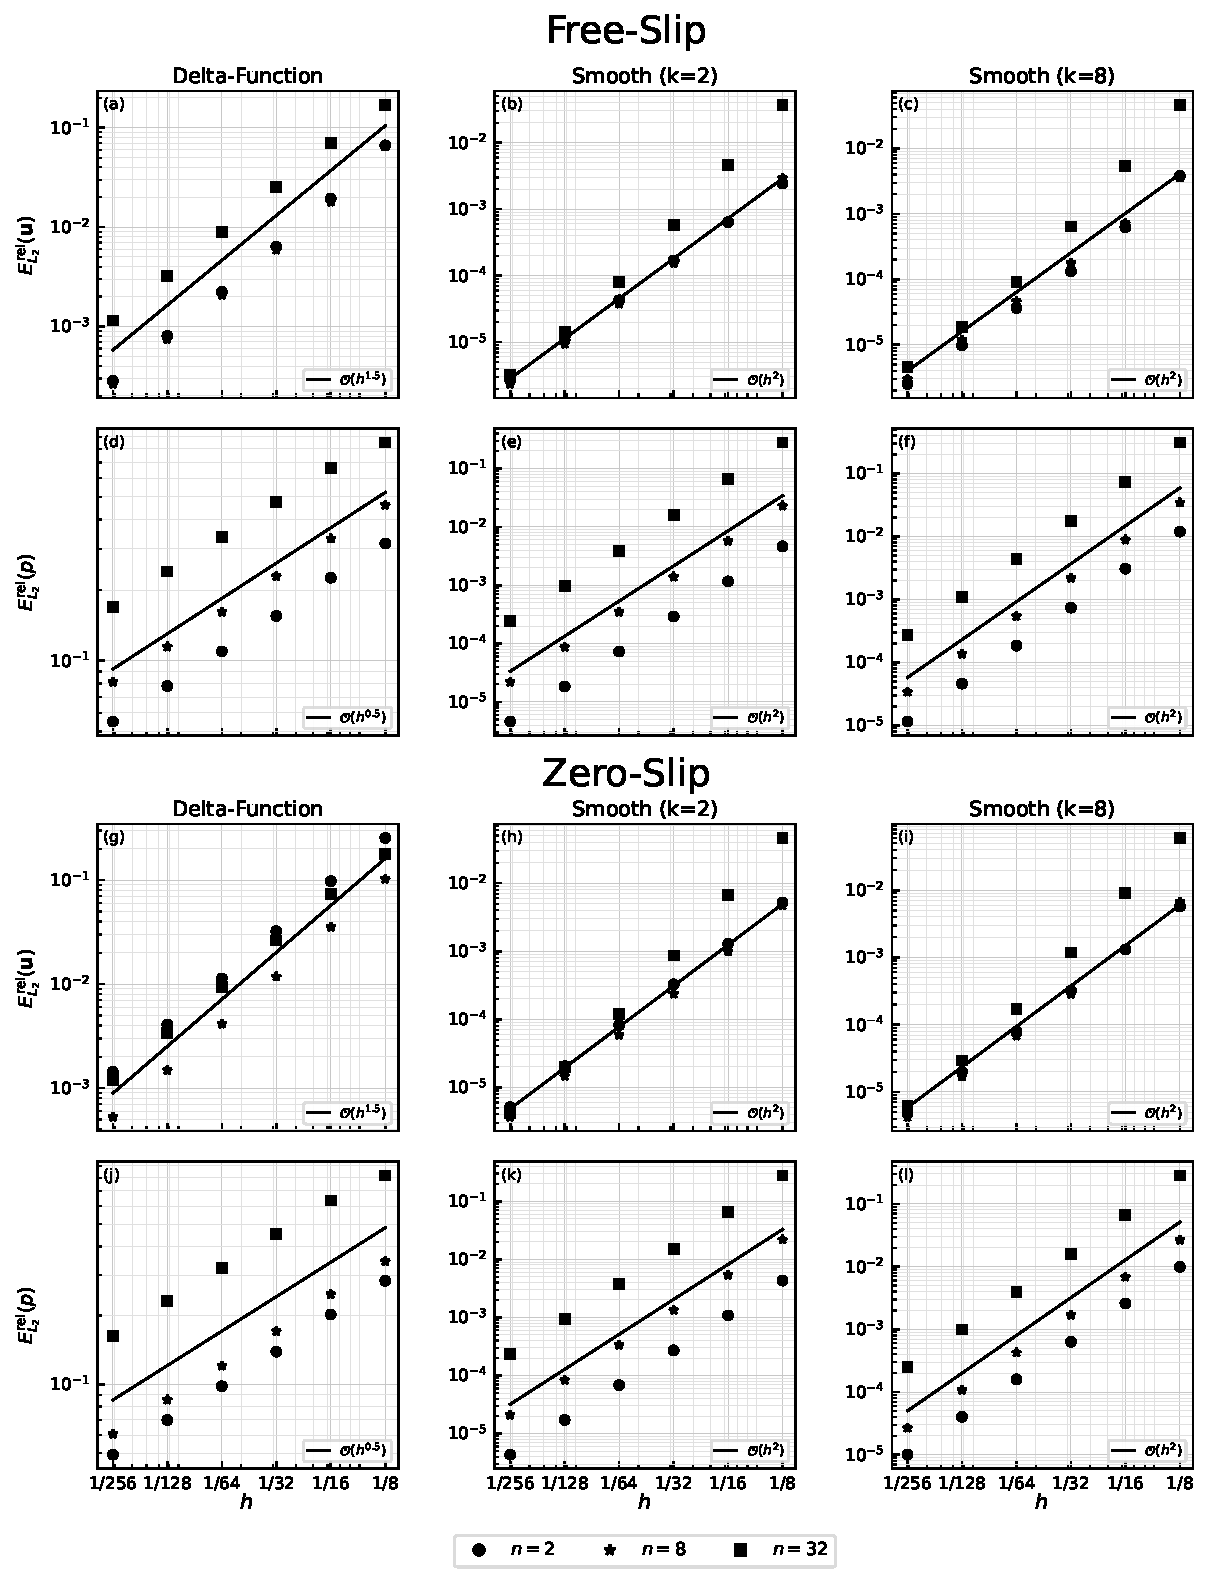
\includegraphics[width=0.82\linewidth]{figure_3_kramer_annulus_convergence.pdf}
    \caption{Velocity and pressure convergence for the four Kramer annulus
    cases. Columns show delta-function forcing and smooth forcing with \(k=2\)
    and \(k=8\). The upper block uses free-slip boundaries and the lower block
    uses zero-slip boundaries.}
    \label{fig:convergence}
\end{figure}

The numerical errors and pairwise convergence rates are provided in Tables~\ref{tab:kramer_annulus_convergence_start}--\ref{tab:kramer_annulus_convergence_end}. Each table groups three azimuthal wavenumbers and reports mesh size, velocity error, velocity rate, pressure error, and pressure rate.

\begin{benchmarklandscape}
\begin{table}[p]
\centering
\caption{Free-slip, delta-function forcing.}
\label{tab:kramer_annulus_convergence_start}
\benchmarktablefont
\setlength{\tabcolsep}{3.2pt}
\fitwidth{%
\begin{tabular}{ccccccccccccc}
\toprule
\multirow{2}{*}{$h$} & \multicolumn{4}{c}{$n=2$} & \multicolumn{4}{c}{$n=8$} & \multicolumn{4}{c}{$n=32$} \\
\cmidrule(lr){2-5}
\cmidrule(lr){6-9}
\cmidrule(lr){10-13}
 & $E_{L_2}^{\mathrm{rel}}(\mathbf{u})$ & rate & $E_{L_2}^{\mathrm{rel}}(p)$ & rate & $E_{L_2}^{\mathrm{rel}}(\mathbf{u})$ & rate & $E_{L_2}^{\mathrm{rel}}(p)$ & rate & $E_{L_2}^{\mathrm{rel}}(\mathbf{u})$ & rate & $E_{L_2}^{\mathrm{rel}}(p)$ & rate \\
\midrule
$1/8$ & \num{6.636e-02} & -- & \num{3.161e-01} & -- & \num{6.455e-02} & -- & \num{4.610e-01} & -- & \num{1.700e-01} & -- & \num{8.511e-01} & -- \\
$1/16$ & \num{1.936e-02} & 1.78 & \num{2.260e-01} & 0.48 & \num{1.798e-02} & 1.84 & \num{3.318e-01} & 0.47 & \num{7.045e-02} & 1.27 & \num{6.624e-01} & 0.36 \\
$1/32$ & \num{6.346e-03} & 1.61 & \num{1.553e-01} & 0.54 & \num{5.914e-03} & 1.60 & \num{2.290e-01} & 0.54 & \num{2.523e-02} & 1.48 & \num{4.736e-01} & 0.48 \\
$1/64$ & \num{2.230e-03} & 1.51 & \num{1.097e-01} & 0.50 & \num{2.084e-03} & 1.50 & \num{1.617e-01} & 0.50 & \num{8.968e-03} & 1.49 & \num{3.364e-01} & 0.49 \\
$1/128$ & \num{8.026e-04} & 1.47 & \num{7.804e-02} & 0.49 & \num{7.460e-04} & 1.48 & \num{1.149e-01} & 0.49 & \num{3.242e-03} & 1.47 & \num{2.400e-01} & 0.49 \\
$1/256$ & \num{2.828e-04} & 1.50 & \num{5.512e-02} & 0.50 & \num{2.643e-04} & 1.50 & \num{8.132e-02} & 0.50 & \num{1.150e-03} & 1.50 & \num{1.699e-01} & 0.50 \\
\bottomrule
\end{tabular}%
}
\end{table}

\begin{table}[p]
\centering
\caption{Free-slip, smooth forcing ($k=2$).}
\benchmarktablefont
\setlength{\tabcolsep}{3.2pt}
\fitwidth{%
\begin{tabular}{ccccccccccccc}
\toprule
\multirow{2}{*}{$h$} & \multicolumn{4}{c}{$n=2$} & \multicolumn{4}{c}{$n=8$} & \multicolumn{4}{c}{$n=32$} \\
\cmidrule(lr){2-5}
\cmidrule(lr){6-9}
\cmidrule(lr){10-13}
 & $E_{L_2}^{\mathrm{rel}}(\mathbf{u})$ & rate & $E_{L_2}^{\mathrm{rel}}(p)$ & rate & $E_{L_2}^{\mathrm{rel}}(\mathbf{u})$ & rate & $E_{L_2}^{\mathrm{rel}}(p)$ & rate & $E_{L_2}^{\mathrm{rel}}(\mathbf{u})$ & rate & $E_{L_2}^{\mathrm{rel}}(p)$ & rate \\
\midrule
$1/8$ & \num{2.441e-03} & -- & \num{4.639e-03} & -- & \num{2.935e-03} & -- & \num{2.313e-02} & -- & \num{3.710e-02} & -- & \num{2.796e-01} & -- \\
$1/16$ & \num{6.377e-04} & 1.94 & \num{1.164e-03} & 2.00 & \num{6.481e-04} & 2.18 & \num{5.728e-03} & 2.01 & \num{4.628e-03} & 3.00 & \num{6.660e-02} & 2.07 \\
$1/32$ & \num{1.680e-04} & 1.92 & \num{2.911e-04} & 2.00 & \num{1.547e-04} & 2.07 & \num{1.401e-03} & 2.03 & \num{5.784e-04} & 3.00 & \num{1.580e-02} & 2.08 \\
$1/64$ & \num{4.260e-05} & 1.98 & \num{7.312e-05} & 1.99 & \num{3.792e-05} & 2.03 & \num{3.487e-04} & 2.01 & \num{7.999e-05} & 2.85 & \num{3.904e-03} & 2.02 \\
$1/128$ & \num{1.076e-05} & 1.99 & \num{1.836e-05} & 1.99 & \num{9.436e-06} & 2.01 & \num{8.722e-05} & 2.00 & \num{1.438e-05} & 2.48 & \num{9.718e-04} & 2.01 \\
$1/256$ & \num{2.704e-06} & 1.99 & \num{4.611e-06} & 1.99 & \num{2.359e-06} & 2.00 & \num{2.189e-05} & 1.99 & \num{3.209e-06} & 2.16 & \num{2.425e-04} & 2.00 \\
\bottomrule
\end{tabular}%
}
\end{table}

\begin{table}[p]
\centering
\caption{Free-slip, smooth forcing ($k=8$).}
\benchmarktablefont
\setlength{\tabcolsep}{3.2pt}
\fitwidth{%
\begin{tabular}{ccccccccccccc}
\toprule
\multirow{2}{*}{$h$} & \multicolumn{4}{c}{$n=2$} & \multicolumn{4}{c}{$n=8$} & \multicolumn{4}{c}{$n=32$} \\
\cmidrule(lr){2-5}
\cmidrule(lr){6-9}
\cmidrule(lr){10-13}
 & $E_{L_2}^{\mathrm{rel}}(\mathbf{u})$ & rate & $E_{L_2}^{\mathrm{rel}}(p)$ & rate & $E_{L_2}^{\mathrm{rel}}(\mathbf{u})$ & rate & $E_{L_2}^{\mathrm{rel}}(p)$ & rate & $E_{L_2}^{\mathrm{rel}}(\mathbf{u})$ & rate & $E_{L_2}^{\mathrm{rel}}(p)$ & rate \\
\midrule
$1/8$ & \num{3.794e-03} & -- & \num{1.195e-02} & -- & \num{3.584e-03} & -- & \num{3.454e-02} & -- & \num{4.638e-02} & -- & \num{3.106e-01} & -- \\
$1/16$ & \num{6.230e-04} & 2.61 & \num{3.080e-03} & 1.96 & \num{7.176e-04} & 2.32 & \num{8.903e-03} & 1.96 & \num{5.447e-03} & 3.09 & \num{7.427e-02} & 2.06 \\
$1/32$ & \num{1.320e-04} & 2.24 & \num{7.416e-04} & 2.05 & \num{1.772e-04} & 2.02 & \num{2.180e-03} & 2.03 & \num{6.411e-04} & 3.09 & \num{1.777e-02} & 2.06 \\
$1/64$ & \num{3.650e-05} & 1.85 & \num{1.848e-04} & 2.00 & \num{4.601e-05} & 1.95 & \num{5.461e-04} & 2.00 & \num{9.064e-05} & 2.82 & \num{4.427e-03} & 2.00 \\
$1/128$ & \num{9.792e-06} & 1.90 & \num{4.617e-05} & 2.00 & \num{1.177e-05} & 1.97 & \num{1.367e-04} & 2.00 & \num{1.858e-05} & 2.29 & \num{1.105e-03} & 2.00 \\
$1/256$ & \num{2.524e-06} & 1.96 & \num{1.154e-05} & 2.00 & \num{3.023e-06} & 1.96 & \num{3.424e-05} & 2.00 & \num{4.520e-06} & 2.04 & \num{2.761e-04} & 2.00 \\
\bottomrule
\end{tabular}%
}
\end{table}

\begin{table}[p]
\centering
\caption{Zero-slip, delta-function forcing.}
\benchmarktablefont
\setlength{\tabcolsep}{3.2pt}
\fitwidth{%
\begin{tabular}{ccccccccccccc}
\toprule
\multirow{2}{*}{$h$} & \multicolumn{4}{c}{$n=2$} & \multicolumn{4}{c}{$n=8$} & \multicolumn{4}{c}{$n=32$} \\
\cmidrule(lr){2-5}
\cmidrule(lr){6-9}
\cmidrule(lr){10-13}
 & $E_{L_2}^{\mathrm{rel}}(\mathbf{u})$ & rate & $E_{L_2}^{\mathrm{rel}}(p)$ & rate & $E_{L_2}^{\mathrm{rel}}(\mathbf{u})$ & rate & $E_{L_2}^{\mathrm{rel}}(p)$ & rate & $E_{L_2}^{\mathrm{rel}}(\mathbf{u})$ & rate & $E_{L_2}^{\mathrm{rel}}(p)$ & rate \\
\midrule
$1/8$ & \num{2.545e-01} & -- & \num{2.832e-01} & -- & \num{1.025e-01} & -- & \num{3.449e-01} & -- & \num{1.783e-01} & -- & \num{8.167e-01} & -- \\
$1/16$ & \num{9.755e-02} & 1.38 & \num{2.019e-01} & 0.49 & \num{3.555e-02} & 1.53 & \num{2.473e-01} & 0.48 & \num{7.344e-02} & 1.28 & \num{6.355e-01} & 0.36 \\
$1/32$ & \num{3.228e-02} & 1.60 & \num{1.388e-01} & 0.54 & \num{1.181e-02} & 1.59 & \num{1.707e-01} & 0.54 & \num{2.629e-02} & 1.48 & \num{4.544e-01} & 0.48 \\
$1/64$ & \num{1.134e-02} & 1.51 & \num{9.797e-02} & 0.50 & \num{4.163e-03} & 1.50 & \num{1.205e-01} & 0.50 & \num{9.343e-03} & 1.49 & \num{3.228e-01} & 0.49 \\
$1/128$ & \num{4.083e-03} & 1.47 & \num{6.972e-02} & 0.49 & \num{1.490e-03} & 1.48 & \num{8.563e-02} & 0.49 & \num{3.378e-03} & 1.47 & \num{2.302e-01} & 0.49 \\
$1/256$ & \num{1.439e-03} & 1.50 & \num{4.924e-02} & 0.50 & \num{5.281e-04} & 1.50 & \num{6.061e-02} & 0.50 & \num{1.198e-03} & 1.50 & \num{1.630e-01} & 0.50 \\
\bottomrule
\end{tabular}%
}
\end{table}

\begin{table}[p]
\centering
\caption{Zero-slip, smooth forcing ($k=2$).}
\benchmarktablefont
\setlength{\tabcolsep}{3.2pt}
\fitwidth{%
\begin{tabular}{ccccccccccccc}
\toprule
\multirow{2}{*}{$h$} & \multicolumn{4}{c}{$n=2$} & \multicolumn{4}{c}{$n=8$} & \multicolumn{4}{c}{$n=32$} \\
\cmidrule(lr){2-5}
\cmidrule(lr){6-9}
\cmidrule(lr){10-13}
 & $E_{L_2}^{\mathrm{rel}}(\mathbf{u})$ & rate & $E_{L_2}^{\mathrm{rel}}(p)$ & rate & $E_{L_2}^{\mathrm{rel}}(\mathbf{u})$ & rate & $E_{L_2}^{\mathrm{rel}}(p)$ & rate & $E_{L_2}^{\mathrm{rel}}(\mathbf{u})$ & rate & $E_{L_2}^{\mathrm{rel}}(p)$ & rate \\
\midrule
$1/8$ & \num{5.169e-03} & -- & \num{4.309e-03} & -- & \num{4.692e-03} & -- & \num{2.188e-02} & -- & \num{4.621e-02} & -- & \num{2.766e-01} & -- \\
$1/16$ & \num{1.287e-03} & 2.01 & \num{1.083e-03} & 1.99 & \num{9.929e-04} & 2.24 & \num{5.433e-03} & 2.01 & \num{6.648e-03} & 2.80 & \num{6.437e-02} & 2.10 \\
$1/32$ & \num{3.253e-04} & 1.98 & \num{2.715e-04} & 2.00 & \num{2.375e-04} & 2.06 & \num{1.343e-03} & 2.02 & \num{8.624e-04} & 2.95 & \num{1.527e-02} & 2.08 \\
$1/64$ & \num{8.137e-05} & 2.00 & \num{6.831e-05} & 1.99 & \num{5.873e-05} & 2.02 & \num{3.358e-04} & 2.00 & \num{1.206e-04} & 2.84 & \num{3.784e-03} & 2.01 \\
$1/128$ & \num{2.041e-05} & 2.00 & \num{1.721e-05} & 1.99 & \num{1.467e-05} & 2.00 & \num{8.419e-05} & 2.00 & \num{2.004e-05} & 2.59 & \num{9.432e-04} & 2.00 \\
$1/256$ & \num{5.103e-06} & 2.00 & \num{4.351e-06} & 1.98 & \num{3.662e-06} & 2.00 & \num{2.111e-05} & 2.00 & \num{4.126e-06} & 2.28 & \num{2.354e-04} & 2.00 \\
\bottomrule
\end{tabular}%
}
\end{table}

\begin{table}[p]
\centering
\caption{Zero-slip, smooth forcing ($k=8$).}
\label{tab:kramer_annulus_convergence_end}
\benchmarktablefont
\setlength{\tabcolsep}{3.2pt}
\fitwidth{%
\begin{tabular}{ccccccccccccc}
\toprule
\multirow{2}{*}{$h$} & \multicolumn{4}{c}{$n=2$} & \multicolumn{4}{c}{$n=8$} & \multicolumn{4}{c}{$n=32$} \\
\cmidrule(lr){2-5}
\cmidrule(lr){6-9}
\cmidrule(lr){10-13}
 & $E_{L_2}^{\mathrm{rel}}(\mathbf{u})$ & rate & $E_{L_2}^{\mathrm{rel}}(p)$ & rate & $E_{L_2}^{\mathrm{rel}}(\mathbf{u})$ & rate & $E_{L_2}^{\mathrm{rel}}(p)$ & rate & $E_{L_2}^{\mathrm{rel}}(\mathbf{u})$ & rate & $E_{L_2}^{\mathrm{rel}}(p)$ & rate \\
\midrule
$1/8$ & \num{5.720e-03} & -- & \num{9.905e-03} & -- & \num{6.657e-03} & -- & \num{2.663e-02} & -- & \num{6.009e-02} & -- & \num{2.829e-01} & -- \\
$1/16$ & \num{1.311e-03} & 2.13 & \num{2.585e-03} & 1.94 & \num{1.283e-03} & 2.38 & \num{6.863e-03} & 1.96 & \num{9.136e-03} & 2.72 & \num{6.628e-02} & 2.09 \\
$1/32$ & \num{3.202e-04} & 2.03 & \num{6.338e-04} & 2.03 & \num{2.837e-04} & 2.18 & \num{1.696e-03} & 2.02 & \num{1.185e-03} & 2.95 & \num{1.590e-02} & 2.06 \\
$1/64$ & \num{7.962e-05} & 2.01 & \num{1.596e-04} & 1.99 & \num{6.861e-05} & 2.05 & \num{4.264e-04} & 1.99 & \num{1.699e-04} & 2.80 & \num{3.969e-03} & 2.00 \\
$1/128$ & \num{1.990e-05} & 2.00 & \num{4.003e-05} & 2.00 & \num{1.700e-05} & 2.01 & \num{1.069e-04} & 2.00 & \num{2.923e-05} & 2.54 & \num{9.910e-04} & 2.00 \\
$1/256$ & \num{4.970e-06} & 2.00 & \num{1.003e-05} & 2.00 & \num{4.234e-06} & 2.01 & \num{2.680e-05} & 2.00 & \num{6.181e-06} & 2.24 & \num{2.476e-04} & 2.00 \\
\bottomrule
\end{tabular}%
}
\end{table}
\end{benchmarklandscape}

\section{Discussion}

The convergence behaviour separates primarily by forcing type. Smooth forcing
preserves the regularity needed for second-order pressure convergence with the
\(P_2\times P_1\) discretisation. Velocity convergence is also regular, although
the observed rates are influenced by the curved geometry, boundary-condition
enforcement, and the number of elements per azimuthal wavelength. These effects
are most visible for \(n=32\), where the coarsest meshes under-resolve the
angular structure.

The delta-function cases are more demanding because the forcing is concentrated
on an internal circular interface. The slower convergence rates are consistent
with the reference Kramer solutions and with the expectation that pressure is
especially sensitive to reduced regularity in mixed Stokes discretisations.
Importantly, the free-slip and zero-slip variants show the same qualitative
rates, indicating that the UW3 boundary-condition implementations behave
consistently across both benchmark families.

The benchmark is therefore a useful intermediate verification problem between
Cartesian manufactured solutions and full spherical-shell mantle-convection
calculations. It tests curved-domain Stokes assembly, pressure normalisation,
boundary conditions, and both smooth and non-smooth buoyancy forcing while
remaining compact enough for routine convergence testing.

\conclusions

We have presented a Copernicus-style summary of the UW3 Kramer annulus Stokes
benchmark. The main findings are:
\begin{enumerate}
  \item UW3 reproduces the analytical annulus solutions of \citet{kramer2021}
  for both free-slip and zero-slip velocity boundary conditions.
  \item Smooth forcing cases show approximately second-order pressure
  convergence and systematic second-order or better velocity convergence over
  the tested mesh sequence.
  \item Delta-function forcing cases show the expected reduced convergence,
  approximately \(O(h^{1.5})\) in velocity and \(O(h^{0.5})\) in pressure.
  \item The observed distinction between smooth and interface-localised forcing
  reflects benchmark solution regularity and provides a useful test of finite
  element behaviour in curved geodynamic domains.
\end{enumerate}

These results verify the UW3 implementation for cylindrical-shell Stokes flow
with analytical Kramer forcing and provide a compact reference for future
annulus and spherical-shell benchmark comparisons.

\bibliographystyle{copernicus}
\bibliography{kramer_annulus_benchmark_article_refs}

\end{document}
